% Chapter 2
\chapter{Literature Review Methodology} % Main chapter title

\label{Chapter2} % For referencing the chapter elsewhere, use \ref{Chapter1} 

In this study, we plan to address half of the research questions through a literature review. Hence, we decided to follow a structured and systematic way of reviewing literature. 

A systematic literature review is one type of literature review that has a formal and structured procedure to synthesize the knowledge of existing research studies that are relevant to answer a pre-defined research questions \cite{kofod-petersen_how_nodate, kitchenham_guidelines_2007}. It allows us to understand the current state of the literature and identify research gaps\cite{carrera-rivera_how-conduct_2022}. 

This systematic literature review has two main objectives. First, to identify existing solutions that leverage Digital Twin to enhance security principles for IoT applications. As an extension and subsection of this objective, the concrete concept of the Digital Twin will be synthesised on the way. Second, to identify research studies conducted on the matter of establishing a secure communication channel between Digital Twin and Iot through cryptographic authentication mechanisms.  

We adopted Kitchenham and Charter three phases of performing systematic literature review; namely, planning protocol, conducting review, and reporting review. Basing this guideline and other resources, we created flow diagram for conducting review process. The flow diagram of the scheme is depicted in Figure \ref{fig:slr-proc}. 

\begin{figure}[H]
    \centering
    \includesvg[width=1\textwidth]{images/svg/slrmethoddiagram.svg}
    \caption{Scheme of 2nd stage (conducting review) }
    \label{fig:slr-proc}
\end{figure}


To automate the systematic literature review process, from defining the PICOC to data extraction, we use a web tool called \textit{parsif.al}\footnote{\href{https://parsif.al}{Parsifal} is an online tool designed to support researchers in performing systematic literature reviews within the context of software engineering. Geographically distributed researchers can work together within a shared workspace, designing the protocol and conducting the research}

\section{Review Protocol}

% \subsection{PICOC and Synonyms}
%----------------------------------------------------------------------------------------
% ======================================================================================================
% NOTES, TODOS
% ======================================================================================================

\subsection{Defining PICOC}
PICOC stands for Population, Intervention, Comparison, Output and Context. It is a widely used technique in medical and social science studies to define the focus of a research \cite{carrera-rivera_how-conduct_2022}. However, Kitchenham and Charter  in \cite{carrera-rivera_how-conduct_2022} and Carrera in \cite{kitchenham_guidelines_2007} showed that this technique can also be applied for computer science related research to formulate and structure research questions. 

In this subsection, we define our PICOC criteria for this systematic literature review as follow:-

\textit{Population:} The motivation to conduct this research is the security related problem we identified in the communication between Digital Twin and constrained  (I)IoT devices deployed in the smart industry to collect sensor data. Hence, the problem domain or "Population" for this research is (I)IoT devices used with Digital Twin to enhance security in Industry 4.0. Industries that use Digital Twin and (I)IoT devices, such as smart cities, smart homes, smart grids, smart health, smart manufacturing, etc. In this sense, the "Population" part of PICOC in this review refers to the following terms: Digital Twin, (Industrial)Internet of Things, Industry 4.0, Smart Manufacturing, Cyber-physical Systems, and Critical Infrastructure. 

\textit{Intervention:} Our intervention to address the aforementioned problem - the security issue of digital communication between Digital Twin and (I)IoT - is to implement a lightweight NIST standard cryptographic authentication/encryption scheme for power, storage and computation constraint (I)IoT devices. In this regard, we use the term "authentication" as an intervention.

\textit{Comparison:} Before designing and implementing an intervention for a specific problem, it is important to identify the existing solution in the literature. The results of reviewing, comparing and analysing the existing solution discussed in the relevant research literature can be used as input to design and implement the intervention methodology. With this regard, this study will identify and compare authentication schemes or security mechanisms used in securing a data flow between Digital Twin and (I)IoT. 

\textit{Outcome:} This study has two broad categories of outcomes. The expected outcome of the literature review is to provide insight into the potential benefits of DT in securing (I)IoT applications in Industry 4.0. From a technical implementation perspective, the expected outcome is a bidirectional secure remote access between DT and (I)IoT and ensuring data integrity and a secure communication channel with an efficient and performant cryptographic authentication and encryption scheme for constrained devices.\\

\textit{Context:} This systematic literature review is focused on the Industry 4.0 environment, targeting Digital Twin solutions deployed in smart industries to enhance security. On the other hand, the second part of this study is focused on implementing authentication/encryption algorithms in constrained physical device to measure and compare the performance of lightweight and traditional algorithms in terms of power consumption, execution time and memory usage. 
%----------------------------------------------------------------------------------------


% \subsection{Research Questions}
%----------------------------------------------------------------------------------------
% ======================================================================================================
% NOTES, TODOS
% ======================================================================================================

\subsection{Research Question}
Before beginning the process of study identification and data extraction, it is crucial to identify and clearly define a research question or objectives, as they serve as the guiding principles for conducting a literature review\cite{carrera-rivera_how-conduct_2022}. This systematic literature review aims to address the following research questions:

\begin{itemize}

    % RQ1
    \item \textbf{RQ1: How is Digital Twin used to enhance the security of IoT/IIot applications in the industry 4.0 use cases ?} - 
    this question aims to identify how Digital Twin is used to improving the security of industries that use IoT devices including sensors and actuators to achieve OT (operational technology) security goals: Safety, reliability and availability.
    % \begin{itemize}
    %     % I need a comment from Mohammed on this -> with regad to use case -> is to braod and vogue?
    %     \item \textbf{RQ1.1: What is the concrete concept of Digital Twin} - 
    %     under subcategory of the above research question, the concept of digital and its use cases are explored.
    % \end{itemize}

    % RQ 1
    % \item RQ1. What mututal authentication schemes for DT and IoT application are discussed in the literature? 
    % \item How can we use Digital Twin to enhance security issue in IoT/IIoT application? 
    %  Replace schemes by  mechansims.
    \item \textbf{RQ2: What are the security schemes presented in the literature to ensure the authentication between Digital Twin and its mapped physical devices?} - 
    this question focuses on the identification of authentication mechanisms that are used to ensure the security of DT and (I)IoT communication.
\end{itemize}
%----------------------------------------------------------------------------------------

% \subsection{Key Terms and Search Strategy}
%----------------------------------------------------------------------------------------
% ======================================================================================================
% NOTES, TODOS
% ======================================================================================================
% Define the search strategy for each database if possible 
% Also prepare table with or and operators refer poatek
% I need to modify the title and the resarch question -> Iot to IIoT , the area is in manufcturing or Industry 4.0.
% receive comment on the keyword variants. example IIoT, schemes.
% =======================================================================================================
\subsection{Search keys and Strategies}
Guided by the PICOC criteria and  research questions, we construct four main search strings to create search queries used for each selected databases. These are, "Digital Twin" "IoT" "Authentication", and "Industry". Synonyms, alternative spellings, and similar semantic meanings are considered for each keyword and combined using OR operator. 

During pilot search, on majority of databases, we identified that adding synonyms of "Digital Twin" does not return new paper compared to searching using only the term "Digital Twin". Even though, we included the synonym terms in the table below, we avoided using them during query construction to simplify our search string. 

\begin{table}[h]
% \captionsetup{
%   justification=raggedright,
%   singlelinecheck=false,
%   margin=60pt % adjust margin as needed
% }
% \centering
\caption{ Key terms and key variants.}
\begin{NiceTabular}{p{3.2cm}p{11cm}}
\toprule
    \textbf{Key terms} & \textbf{Variants / Synonyms / Similar Semantic Meaning} \\
    \midrule
    Digital Twin & DT, digital-twin, digital-twins, digital replica, digital shadow, virtual model, virtual clone \\ \hline
    (Industrial)Internet of Things & IoT, IIoT, internet-of-things, internet-of-thing, industrial internet of things, industrial-internet-of-thing, sensors, actuators, smart devices  \\ \hline
    Authentication & security, confidentiality, certificate, verification, scheme, schemes\\ \hline
    Industry & industry 4.0, manufacturing, smart manufacturing, factory, smart factory, cyber-physical system, cyber-physical systems, cyber physical systems, cyber physical system, critical infrastructure, critical infrastructures. \\ 
\bottomrule
\end{NiceTabular}
\end{table}

% As an example, an advance search query for Scopus databases is shown in table \ref{}.\\


% \begin{table}[h]
% % \centering
% \caption{\label{scopus-advanc-search} Example of advanced search query in Scopus}
% \begin{NiceTabular}{Y{1.1}}
% \CodeBefore
%   \rowcolor{gray!50}{1}
%   \rowcolors{2}{gray!25}{white}
% \Body
%  ("dt" OR "digital twin" OR "digital twins" OR "digital-twin" OR "digital-twins" OR "digital replica" OR "digital shadow" OR "virtual model" "virtual clone")  \\
%  AND \\
%  ("internet of things" OR "internet of thing" OR "internet-of-thing" OR "internet-of-things" OR "IIoT" OR "industrial internet of things" OR "industrial-internet-of-thing" OR "sensors" OR "actuators" OR "smart devices" )  \\
%  AND \\
% ("security" OR "authentication" OR "certificate" OR "verification" OR "schemes") \\
%  AND \\
% ("industry" OR "industry 4.0" OR "manufacturing" OR "smart manufacturing" OR "factory" "smart factory" OR "cyber-physical systems" OR "cyber-physical system" OR "cyber physical system")  \\
% \end{NiceTabular}
% \end{table}
%----------------------------------------------------------------------------------------

% \subsection{Digital Library}
%----------------------------------------------------------------------------------------
% ======================================================================================================
% NOTES, TODOS
% ======================================================================================================
% One paragraph about the databases 
% A table that show description and reason for selection
\subsection{Digital Library Sources}

To conduct a comprehensive literature review relevant to our research question, we utilised six electronic databases renowned for publishing computer science research papers. Of these six databases, we selected four, namely ScienceDirect, Scopus, IEEExplore, and ACM, adhering to the recommendation by  Brereton et al. \cite{BRERETON2007571} cited in Kitchenham and Charter \cite{kitchenham_guidelines_2007}.




%----------------------------------------------------------------------------------------

% \subsection{Inclusion and Exclusion Critera}
%----------------------------------------------------------------------------------------
% ======================================================================================================
% NOTES, TODOS
% ======================================================================================================

\subsection{Inclusion and Exclusion Criteria }
\label{sec:inc-exc}


\textit{Inclusion}: We only considered studies written in English, accessible in full text, and published in journals or conferences in the field of computer science between 2016 and 2022. 

\textit{Exclusion:} Any studies that did not meet the inclusion criteria, including those written in a language other than English, not accessible in full text, papers classified as gray literature, published before 2016, or not related to computer science or our research questions, were excluded from the selection process. The decision to commence our research from the year 2016 was made following a pilot search on prominent academic databases. Our preliminary findings revealed that a significant number of papers, exceeding 20, which incorporate the term "Digital Twin" in their abstracts, keywords, or titles have been published since that year. Another reason is the fact that Digital Twin is a new research topic and growing , most of the relevant papers have been published in the last 6 years. 

The inclusion and exclusion criteria utilized for the purpose of filtering research studies from the search results of databases are presented in Table \ref{tbl:table-inc-exc}. 

\begin{table}[H]
\centering
\caption{\label{tbl:table-inc-exc}Inclusion and exclusion criteria.}
\begin{NiceTabular}{p{3cm}p{6cm}p{5cm}}
\toprule
    \textbf{Criteria Type} & \textbf{Inclusion} & \textbf{Exclusion} \\
    \midrule
    \textbf{Period} & Studies published between 2016 and 2022 & before 2016 \\ 
    \textbf{Language} & English & Not English \\
    \textbf{Accessibility} & accessible in full-text & Not accessible in full-text \\ 
    \textbf{Type of source} & Journal articles, conference proceedings  & Books, book chapter, \\ 
    \textbf{Type of literature} & Of type black literature & Grey literature  \\ 
    \textbf{Relevance} & Study related to computer science & Not related to computer science \\
\bottomrule
\end{NiceTabular}
\end{table}


%----------------------------------------------------------------------------------------

%----------------------------------------------------------------------------------------
% ======================================================================================================
% NOTES, TODOS
% ======================================================================================================
% describe how to perform the detail assessment
% use numeral scale 
% Are the aim of the article clearly stated?
% Is the implementation detail explained adequately 
% does the study has direct link to research question 1 and/or question 2. 
% 
\subsection{Quality Assessment Checklist}
After selecting papers using the inclusion and exclusion criteria, we also evaluate the papers using a quality assessment checklist. This evaluation takes place during the review phase, with the goal of identifying and eliminating articles that fail to meet the checklist criteria. In other words, a paper is removed if it does not satisfy any of the criteria on the checklist.


The quality assessment checklist that defines the detailed assessment criteria is outlined below.
% Besides the inclusion and exclusion criteria, it is important to evaluate the quality of the research study\cite{kitchenham_guidelines_2007}.
\begin{itemize}
    \item \textbf{QA1:} Abstract: Is the research question (the aim) clearly defined and relevant to the field of study?
    \item \textbf{QA2:} Abstract: Does the study propose any new security solutions or improvements to existing ones? ensuring the security (I)IoT application using Digital Twin?
    \item \textbf{QA3:} Methodology: Does the study adequately explain a methodology or framework to secure (I)IoT applications using DT?
    \item \textbf{QA4:} Methodology: Does the study conducted an experiment (test bed) or use case to validate the hypothesis?
    \item \textbf{QA5:}Methodology: Does the study provide detailed procedures to ensure secure communication between DT and IoT?
    \item \textbf{QA5:}Result: Are the results of the study clearly presented and supported by the data?
    \item \textbf{QA5:}Discussion: Does the research provide a discussion and analysis of the implications and potential future work in the field?
\end{itemize}
% The quality assessment questions outlined above were evaluated using a numerical metric scoring system, with a range of 1-5, where 1 represents an irrelevant article and 5 represents a highly relevant and qualified article. The level of agreement in answering the quality checklist questions was determined through a categorical classification system, comprising of "Agree," "Somewhat Agree," "Neutral," "Somewhat Disagree," and "Disagree." These categories were assigned corresponding weight values, with "Agree" being assigned the highest weight value of 5 and "Disagree" being assigned the lowest weight value of 1. This scoring system helped to ensure that we evaluated research studies in a fair and consistent way so that the studies that were the most relevant and of the highest quality were selected for the review.

% The number of articles and their scores is depicted in the diagram [blab bla]. 

%----------------------------------------------------------------------------------------

% \subsection{Defining Data Extraction Form}
%----------------------------------------------------------------------------------------
% ======================================================================================================
% NOTES, TODOS
% ======================================================================================================

\subsection{Data Extraction Form}
According to Kitchenham et al.\cite{kitchenham_guidelines_2007}, a well design data extraction form is crucial for collecting information from selected primary studies to address research questions. In this study we use parsif.al web tool to design and structure data extraction form for collecting data from selected papers.  

The data extraction form is continuously evolving during the full-text review process. 

More data to be filled..... A table with data extraction from will be drawn here. 
%----------------------------------------------------------------------------------------


\section{Conducting Review}
In total, 523 articles have been retrieved from online digital databases -- ScienceDirect, SpringerLink, Scopus, IEEExplore, ACM and WebofScience-- that are well known for publishing research studies related to computer science. 
For all databases, we limit the search result based on the following criteria we defined in section \ref{sec:inc-exc}. Only papers from computer science subject areas are selected. In addition, only document-type articles and papers from journals and conferences of source type are included in the final search result. For each selected database, we employ different search queries and search strategies.

% \subsection{Search Queries and Search Strategy}
%----------------------------------------------------------------------------------------
% ======================================================================================================
% NOTES, TODOS
% ======================================================================================================
\subsection{Search Queries and Search Strategy}

 Each of the selected database comes with their own way of performing advance searching. The search field and filtering option are different from one database to another. Having this into consideration, we design a search strategy we called bottom down three stage searching mechanism. The detail at each stage is explained as follow. 

First we look for the main key term -- Digital twin -- on the title of the paper. The assumption behind this is that if the research main focus is digital twin it is highly likely that its title contains digital twin. Since our main objective is to understand how digital twin is used to secure IoT application on various sectors, we then narrow the previous search result by looking for security related terms such as "authentication", "security", "encryption", and "cryptography" on the abstract. In the third stage, if the number of retrieved papers is greater than 30, we further narrow the search result by tuning our search query to look for IoT and industry related terms in the full text of the research paper. 

\begin{tcolorbox}[colback=black!5!white, sharp corners=all, colframe=white!95!black]
\textbf{Web of Science}
\tcblower
("digital twin*" OR "digital-twin*") (Title) AND ( "authenticat*" OR "cryptography" OR "security" OR "encrypt*" ) (Abstract) and English (Languages) and Article or Proceeding Paper (Document Types) and Engineering or Computer Science (Research Areas)
\end{tcolorbox}

In Web of Science, "Topic"(i.e Title, keyword, and Abstract) filed is used to search for digital twin and internet of things terms. The security related terms like authentication, encryption, cryptography and encryption as well as terms related to industry are searched on all fields. From the search results of our query, document types such as book chapters, early access,and editorial are excluded. In other words, only document of type article and conference papers are selected. We run the search query over all available years which are published under category of computer science and 30 articles are returned as a result.
\begin{tcolorbox}[colback=black!5!white, sharp corners=all, colframe=white!95!black]
\textbf{Scopus}
\tcblower
( TITLE ( ( "digital twin*" OR "digital-twin*" ) ) AND TITLE-ABS-KEY ( "authenticat*" OR "cryptography" OR "security" OR "encrypt*" ) AND TITLE-ABS-KEY ( ( "industr*" OR "Industry 4.0" OR "factor*" OR "manufactur*" OR "smart manufacturing" OR "cyber-physical system*" OR "cyber physical System*" OR "infrastructure*" OR "industrial control system*" ) ) ) AND ( LIMIT-TO ( SUBJAREA , "COMP" ) OR LIMIT-TO ( SUBJAREA , "ENGI" ) ) AND ( LIMIT-TO ( DOCTYPE , "cp" ) OR LIMIT-TO ( DOCTYPE , "ar" ) ) AND ( LIMIT-TO ( SRCTYPE , "p" ) OR LIMIT-TO ( SRCTYPE , "j" ) ) AND ( LIMIT-TO ( LANGUAGE , "English" ) )
\end{tcolorbox}
We employ the same search methodology and search terms for Scopus as we do for Web of Science. We run our query string with intention to find terms in "Article title", "Abstract" and "Keywords". While document type article and conference paper are included; conference review and book chapter are excluded. Our search result returned 97 articles in total. 

\begin{tcolorbox}[colback=black!5!white, sharp corners=all, colframe=white!95!black]
\textbf{IEEExplore}
\tcblower
("Document Title":"digital twin*" OR "Document Title":"digital-twin*") AND ("Abstract":"authenticat*" OR "Abstract":"cryptography" OR "Abstract": "security" OR "Abstract":"encrypt*") \\

Filters Applied: Conferences Journals
\end{tcolorbox}
In the case IEEE, we use a different search strategy from the above two cases. while we perform search for terms  authentication and industry related on full text , the "All Metadata" field is used to perform the others search terms on title, keywords, and abstract. Articles from conferences and journals are selected and articles under category of early access and magazines are excluded. Finally, Our query resulted in 37 research studies.   

\begin{tcolorbox}[colback=black!5!white, sharp corners=all, colframe=white!95!black]
\textbf{ACM}
\tcblower
[[Title: "digital-twin*"] OR [Title: "digital twin*"]] AND [[Abstract: "security"] OR [Abstract: "authenticat*"] OR [Abstract: "encrypt*"] OR [Abstract: "cryptography"]]

\end{tcolorbox}
ACM is a bibliographic database that exclusively focuses on publishing computing literature. In ACM we run the search query within the search field of "Anywhere". And only research articles are included, and as a result 12 research studies are retrieved. 





%----------------------------------------------------------------------------------------


% \subsection{Search Result and Bibliometric Analysis}
%----------------------------------------------------------------------------------------
% ======================================================================================================
% NOTES, TODOS
% ======================================================================================================
\subsection{Search Result and Bibliometric Analysis}

After completion of the selection process, which involved applying inclusion and exclusion criteria and eliminating duplicate studies, a total of 73 research papers were considered eligible for further review and analysis. The accompanying pie chart (see Figure \ref{fig:archive-itemtype}) reveals that IEEE was the primary publisher of the selected papers, accounting for 49 of them. SpringerLink was the second largest contributor, with 14 publications, while Elsevier (4), ACM (3), MDPI (1), Pergamon (1) and SpieDigitalLibrary (1) each account for the lowest contribution of publications. The second right side of the pie chart also demonstrates that the majority of the selected papers were sourced from Web of Science and Scopus, followed by IEEE and SpringerLink. The distribution of publication types among the 73 selected papers is worth nothing. Of these papers, 60\% (i.e., 44 papers) were published as conference papers, whereas the remaining 40\% (i.e., 29 papers) were in the form of journal articles.



% \begin{figure}
% \includesvg[width=0.5\textwidth]{images/svg/databases.svg}
% \includesvg[width=0.5\textwidth]{images/svg/itemtype.svg}
% \svgcaption{This is the label for the SVG image.}
% \label{fig:image}
% \end{figure}

\begin{figure}[H]    
    \caption{An Analysis of Paper Distribution Based on Source and Publisher.}
    % \centring
    \begin{subfigure}[b]{0.45\textwidth}
    \caption{Number of selected papers per publisher.}
        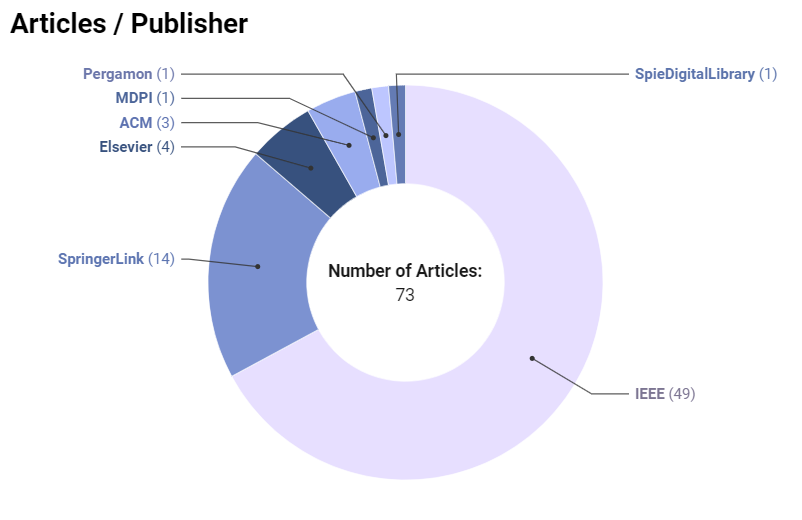
\includegraphics[width=\textwidth]{images/articles_per_publisher_2.png}
        % \includesvg[width=\textwidth]{images/svg/databases.svg}
    \end{subfigure}
    \begin{subfigure}[b]{0.45\textwidth}
    \caption{Number of selected papers per source.}
        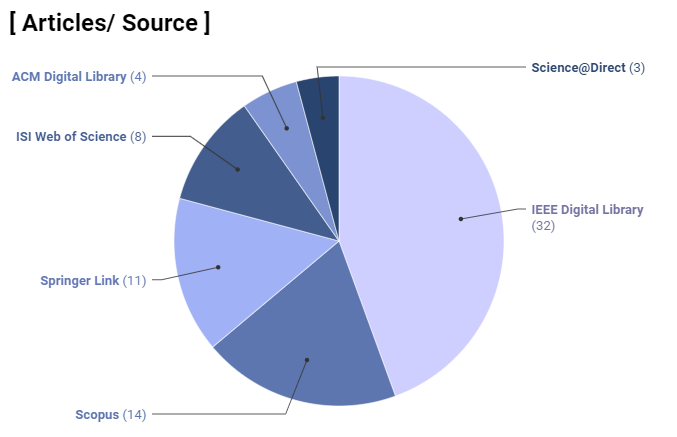
\includegraphics[width=\textwidth]{images/artpersrc_final.png}
        % \includesvg[width=\textwidth]{images/svg/itemtype.svg}
    \end{subfigure}
    \label{fig:archive-itemtype}
\end{figure}
 
Analysis of the distribution of selected papers based on publication year revealed that the majority of articles were published in 2022 and 2021 (see Figure \ref{fig:bar-chart-yaer}). Furthermore, the bar chart illustrates a general upward trend in the number of publications addressing security concerns for industries utilising Digital Twin and (I)IoT applications. This trend indicates that there is a growing interest and concern among researchers in the field of Digital Twin and (I)IoT security, and highlights the relevance of this systematic literature review.

\begin{figure}[H]    
    \caption{Yearly Publication Statistics: Investigating the Number of Papers Published}
    % \includesvg[width=0.9\textwidth]{images/svg/pub_year_white_bg.svg}
    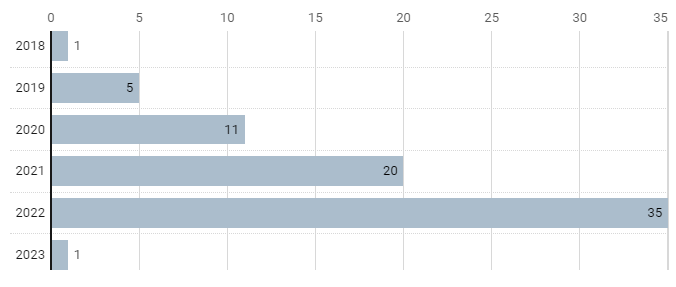
\includegraphics[width=\textwidth]{images/year8.png}
    \label{fig:bar-chart-yaer}
\end{figure}

To gain a deeper understanding of the trending topics within the 73 selected papers published between 2018 and 2023, a frequency analysis of keywords was conducted. This analysis was performed by extracting keywords that appeared more than three times in the abstracts and keyword sections of the articles using the VOSviewer tool. Further filtering and sensitization was applied to create a shortlist of keywords. Additionally, keywords which have similar meanings with different spellings and variations were merged. The resulting frequency analysis of keywords, illustrated in Figure \ref{fig:alluvial-key}, provides valuable insight into the key themes and concepts that are prevalent in current research on the topic of DT and IoT security. This analysis can help guide future research by identifying areas where there is a need for further investigation and providing a sense of the current state of the field.


\begin{figure}[H]
    % \includesvg[width=0.9\textwidth]{images/svg/key_buble.svg}
    % 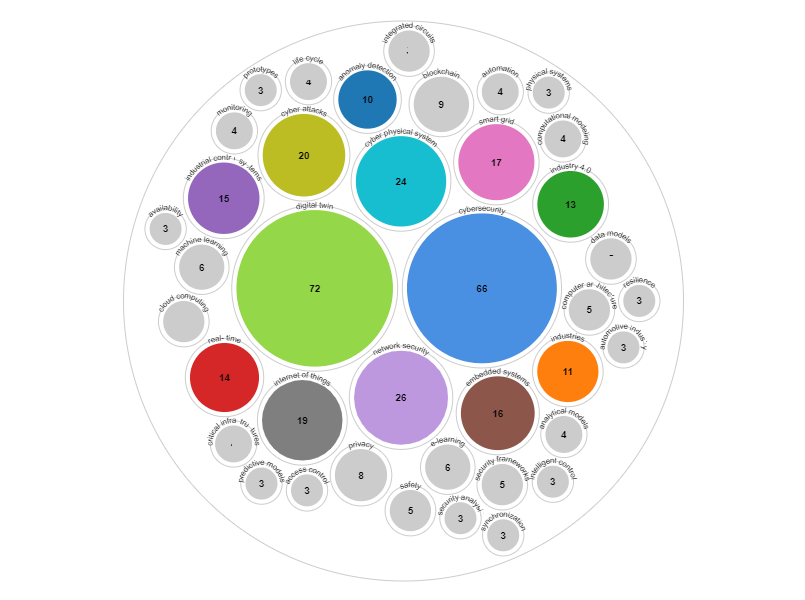
\includegraphics[width=\textwidth]{images/svg/key_buble.png}
    \caption{Frequency of keywords from abstract and keywords of 73 papers}
    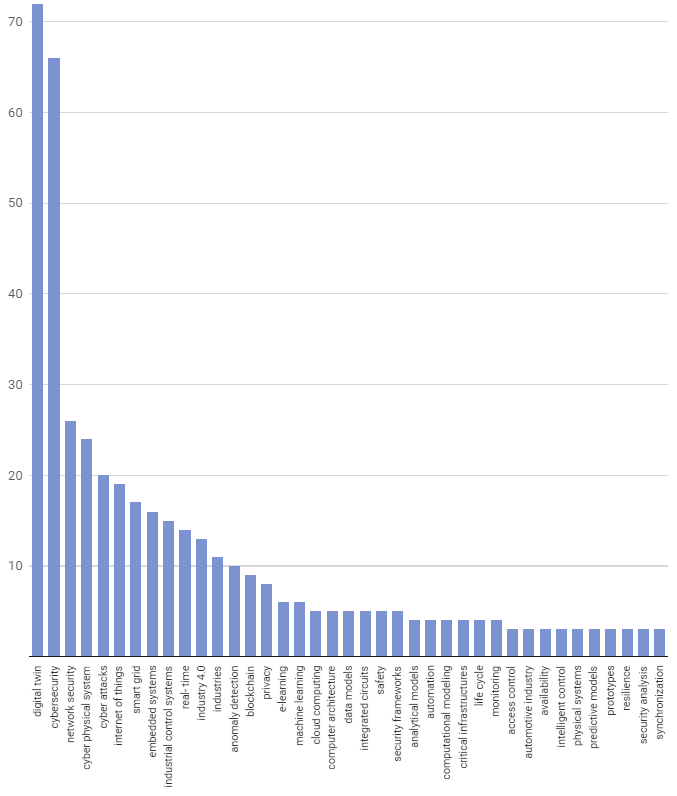
\includegraphics[width=0.8\textwidth]{images/keyword_occurance.png}
    \label{fig:alluvial-key}
\end{figure}
As was previous stated, in this study, 73 papers were analyzed to generate a list of 1187 keywords using VOSViewer. During our analysis, we utilized a thesaurus text file to merge keywords with similar semantic meanings.

For instance, we replaced artificial intelligence and deep learning with machine learning, and intrusion detection with anomaly detection. We also merged related terms such as cyber-attacks, denial-of-service attacks, cyber attacks, and computer crime into a single term - cyber attacks. Similarly, we combined control systems under the term industrial control system and grouped electric power transmission network and smart power grids as smart grid. We further streamlined our findings by using industry 4.0 as an umbrella term for smart manufacturing. Additionally, we have replaced the term "real-time system" with "real-time". 

Moreover, we limited the results to the top 87 keywords that appeared at least 3 times within the original list of 1187 keywords.  


The analysis of the selected papers using VOSviewer software revealed that which terms were frequently mentioned in the abstract and keyword section of the paper. The most frequently mentioned terms were "digital twin" with 72 occurrences, followed by "cybersecurity" with 66 occurrences, "cyberphysical system" with 24 occurrences, "cyber attacks" with 20 occurrences, "internet of things" with 19 occurrences, and "embedded systems" with 17 occurrences. This analysis highlights the key themes and concepts that are prevalent in current research on the topic of Digital Twin and IoT security. The high frequency of the term "digital twin" indicates the centrality of this concept in the field and the importance of understanding its role in ensuring the security of industries utilizing DT and IoT applications. The frequent mention of terms such as "cybersecurity" and "cyber attacks" further emphasizes the need for robust security measures to protect these systems from malicious actors. Additionally, the presence of terms such as "cyberphysical system" and "embedded systems" highlights the need for interdisciplinary research and collaboration between experts in fields such as computer science, engineering, and physics to effectively address the security challenges facing Digital Twin and IoT.

In order to gain further insights into the evolution of research in the field of Digital Twin and IoT security, a keyword co-relationship network analysis was extracted from the VOSviewer tool. This analysis aimed to identify clusters of related items and visualise the relationships between keywords over time. The results of this analysis revealed that in the early days of research on Digital Twin, keywords such as "monitoring", "safety", "prototypes", "resilience", "software", and "tools" were frequently mentioned, which suggests that the primary focus of research at that time was on utilising Digital Twin as a visual aiding tool. However, more recent research is characterized by the frequent mention of emerging technologies such as "blockchain," "machine learning," "e-learning" "5G," and "privacy" This indicates that the development of Digital Twin has shifted towards utilising these technologies and augment Digital Twin to provide more service other than used as a model.



\begin{figure}[H]
    % \centering    
    \caption{keyword co-relationship from VOSviewer}
    % 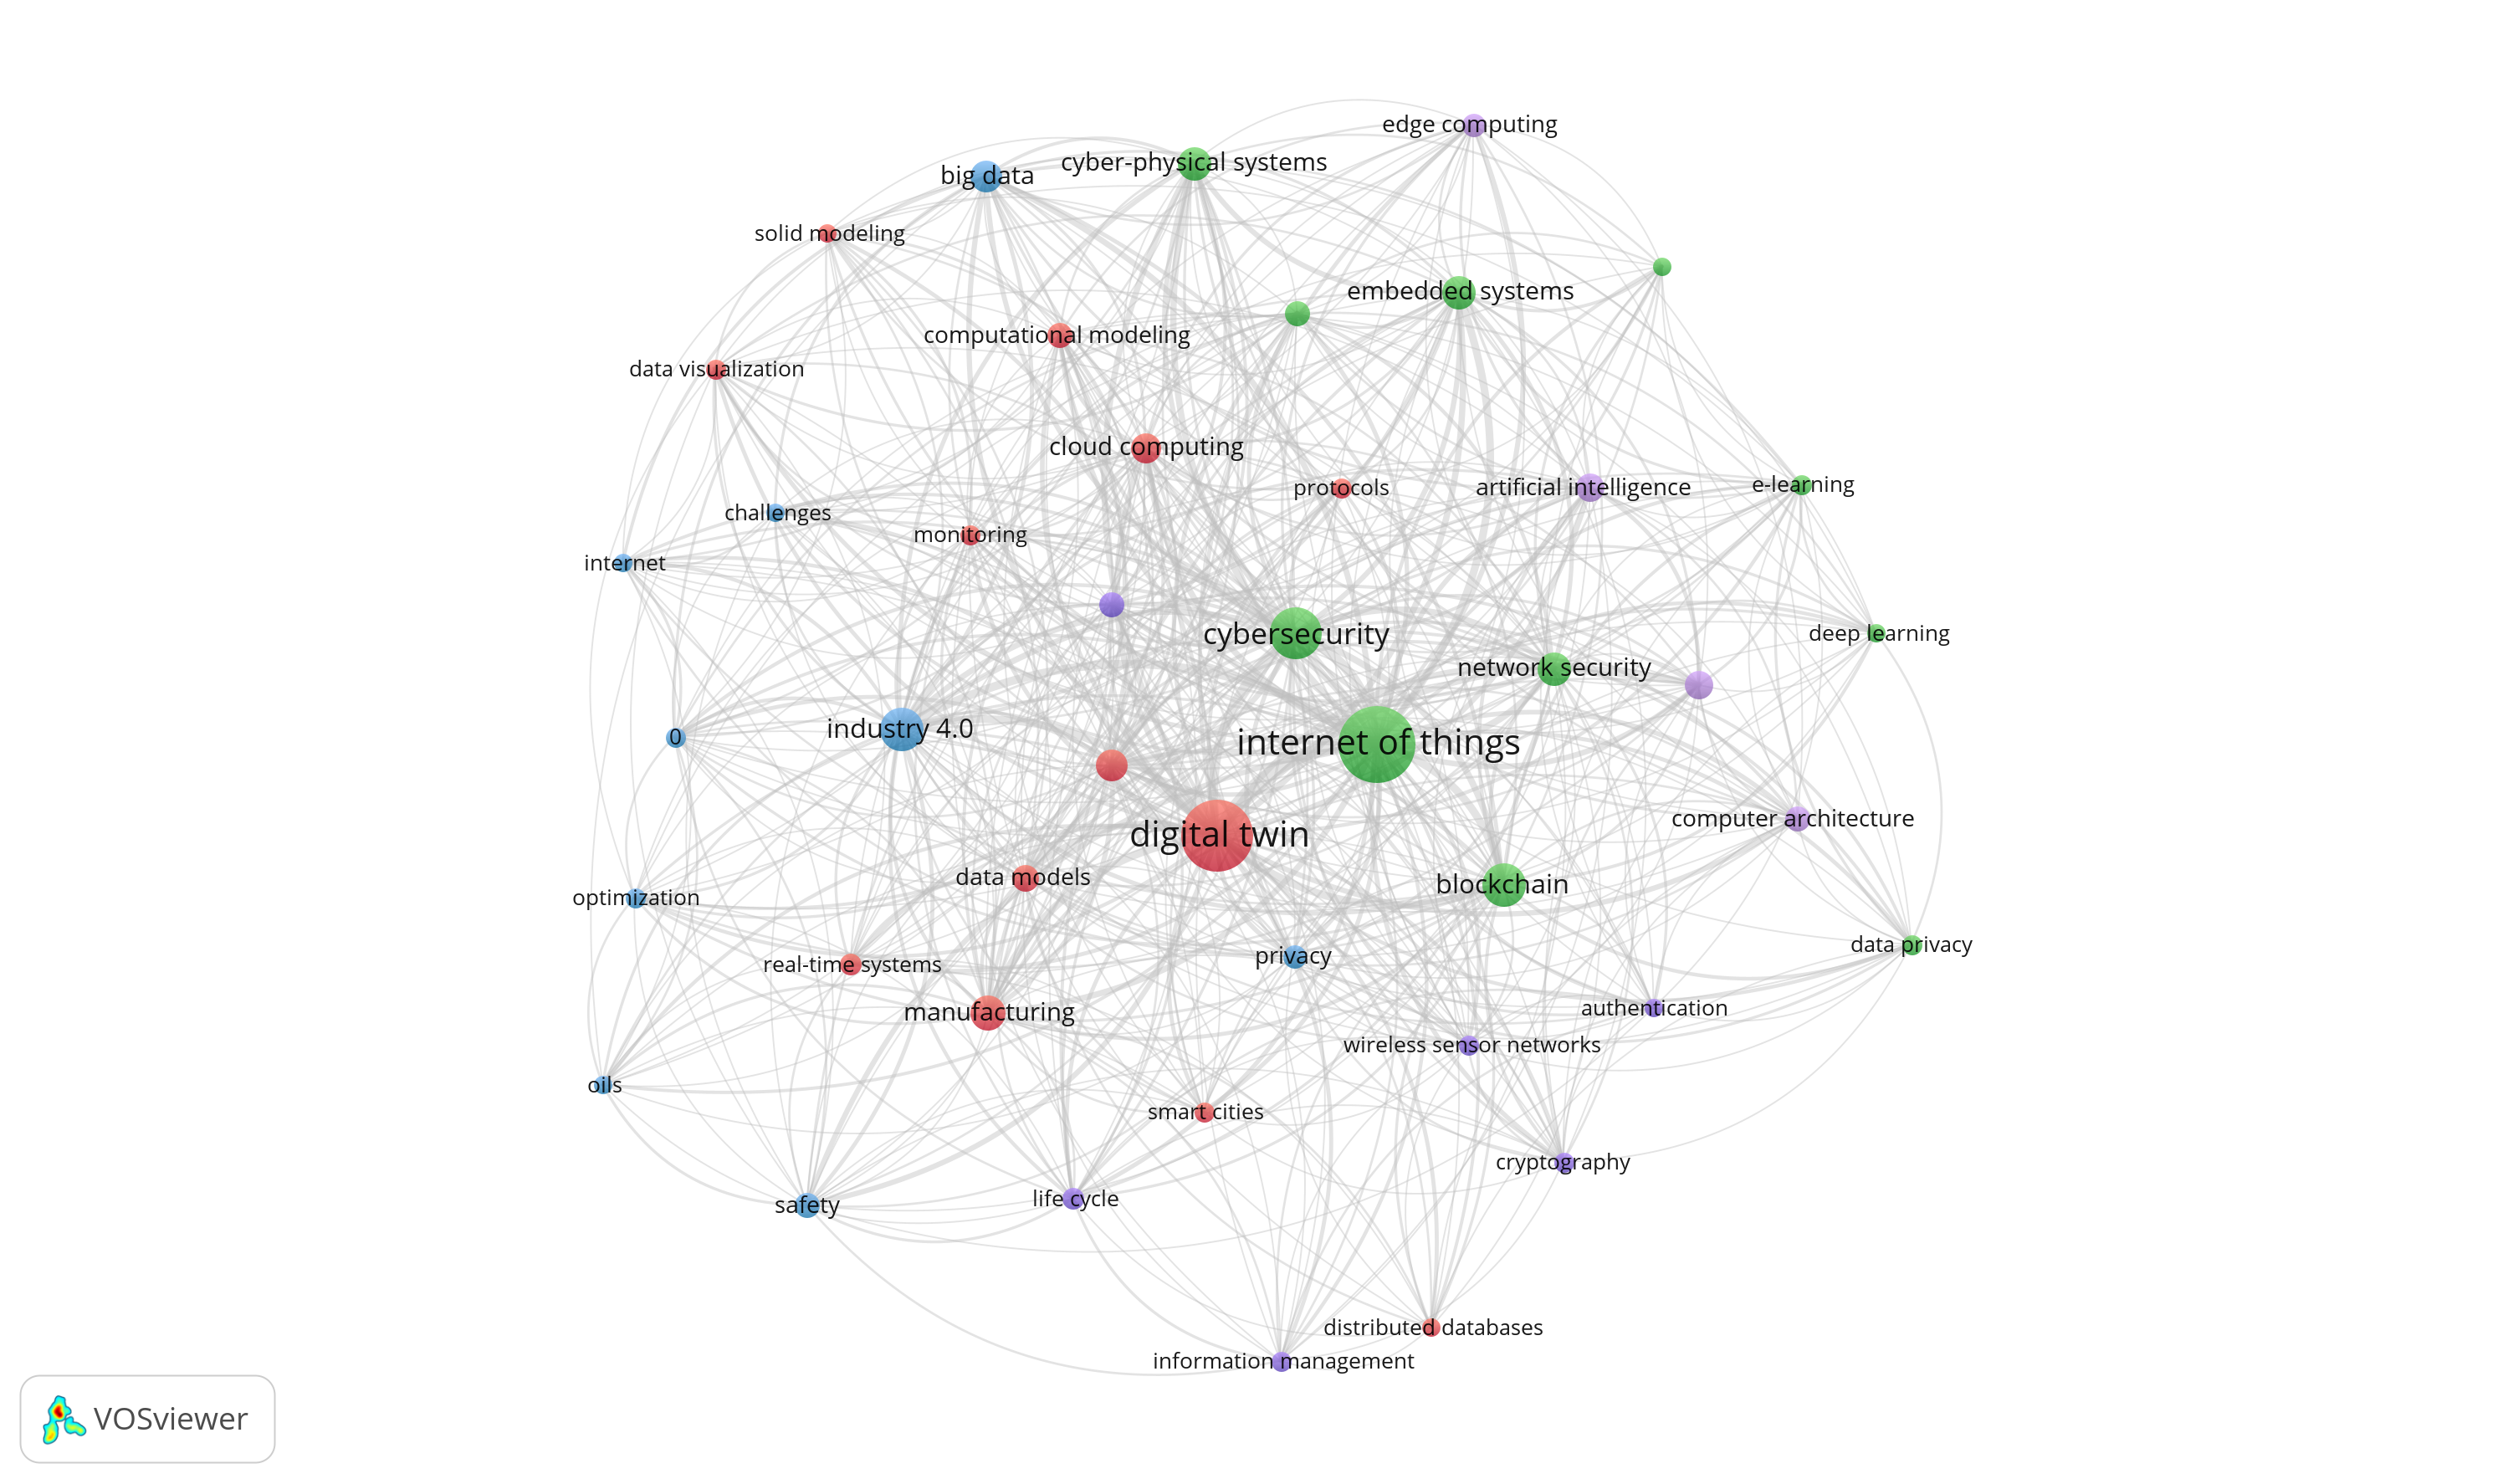
\includegraphics[width=1.5\textwidth, center]{images/vos_key_cooc_6_final.png}
    \includesvg[width=\textwidth]{images/svg/vos_co_time_2.svg}
    % \includesvg[inkscapelatex=false,width=0.95\columnwidth]{images/key_belt.svg}
    \label{fig:co-occurrence-vosv}
\end{figure}

The analysis of the co-occurrence of keywords in the selected articles, as represented in Figure \ref{fig:co-occurrence-vosv}, reveals the identification of five clusters. These clusters, as defined by the VOSviewer documentation, are groups of terms that exhibit a high degree of relatedness. 

Cluster one encompasses terms related to 5G technology, machine learning, real-time security analysis, security frameworks, access control, and automation highlighting the importance of incorporating advanced technologies in the field of security and access control automation. This cluster also suggests a growing emphasis on real-time security analysis to ensure quick identification and response to potential threats

Cluster two comprises keywords such as cybersecurity, data models, digital twin, internet of things, privacy, prototypes, safety, and cloud computing. The inclusion of terms such as privacy, prototypes, and safety in this cluster indicates a growing concern for the protection of sensitive information and the security of digital representations of physical systems. 

The third cluster encompasses terms such as those related to the automotive industry, availability, blockchain, industry 4.0, industrial control systems, system life cycles, intelligent control, software, and tools. This cluster suggests a growing emphasis on the use of blockchain technology for secure data management in the automotive industry for data sharing. 

The fourth cluster is comprised of analytical models, anomaly detection, cyber-attacks, monitoring, resilience, critical infrastructure, integrated circuits, and physical systems. This cluster shows the association of identification and mitigation of potential security threats through the use of analytical models to detect anomalies to increase the resilience of critical infrastructure.

The final cluster includes terms such as cyber-physical systems, e-learning, embedded systems, predictive models, and smart grids. This cluster highlight the importance of training and education to promote the secure use of cyber-physical system such as smart grids.
%----------------------------------------------------------------------------------------

% \subsection{Study Selection and Refinement}
%----------------------------------------------------------------------------------------
% ======================================================================================================
% NOTES, TODOS
% ======================================================================================================
\subsection{Study Selection and Refinement}
% 74 selected papers -> 14 not relevant and 3 duplicate studies submitted to different journals  excluded during full review of the papers. 

After the screening of 452 papers, initially, we were left with 89 papers. However, during the review phase, we exclude 21 papers from our analysis and data extraction. For example, we have found three studies that were duplicated with different metadata but had similar content and had been submitted to different journals. These duplicates were not identified by the tools we had used to exclude them. In addition, through the quality assessment checklist, we also excluded 18 papers for the data extraction phase.

Some of the reasons for the exclusion of these papers were as follows:

\begin{itemize}
    \item When the paper discussed how to secure the digital twin itself, rather than securing IoT applications using digital twin technology or securing the communication channel between DT and (I)IoT. 
    \item If the paper lacked a clear objective and aim.
    \item Some were not related to securing (I)IoT applications with an Industry 4.0 use case (for example, a study that used a digital twin to secure a data centre).
    \item Study sourced from book chapter. 
    \item The study was not relevant to any of the research questions.
    \item A study that focuses on securing (I)IoT devices that are not associated with any industry use case. 
\end{itemize}

As a result of this refinement and selection process, we were left with final set of 69papers that were used for data extraction and analysis. In the following chapter, we provide a review of the 69 papers focusing to answer two research questions: How is digital twin used to improve the security of (I)IoT applications and what security mechanisms are used to secure the communication channel?    




%----------------------------------------------------------------------------------------

% \subsection{Data Extraction and Monitoring}
%----------------------------------------------------------------------------------------
% ======================================================================================================
% NOTES, TODOS
% ======================================================================================================
% \subsection{Data Extraction and Monitoring}
\label{sec:data-ext}
%----------------------------------------------------------------------------------------

% \subsection{Data Synthesis}
%----------------------------------------------------------------------------------------
% ======================================================================================================
% NOTES, TODOS
% ======================================================================================================
% \subsection{Data Synthesis}
%----------------------------------------------------------------------------------------







%----------------------------------------------------------------------------------------

% Todo: Method for data extraction and synthesis 
% \subsection{Data Extraction Method}
% \subsection{Data Synthesis Method}